\documentclass[a4paper,11pt]{article}
\usepackage{pos}

\title{Heavy neutral lepton searches at the LHC}
\ShortTitle{Heavy neutral lepton searches at the LHC}

\author*[a,1]{Matthias Komm}

\affiliation[a]{CERN,\\
  Geneva, Switzerland}
\note{For the ATLAS, CMS, and LHCb collaborations.}

\emailAdd{Matthias.Komm@cern.ch}



\abstract{Models involving heavy neutral leptons offer a compelling explanation of various observed phenomena that are not described by standard model of particle physics. In this note, recent results on searches for heavy neutral leptons in proton-proton collisions by the ATLAS, CMS, and LHCb collaborations are reviewed.
}

\FullConference{%
 The Ninth Annual Conference on Large Hadron Collider Physics - LHCP2021\\
 7-12 June 2021\\
 Online
}

\begin{document}
\maketitle


\section{Introduction}
Heavy neutral leptons (HNLs) can be introduced into the standard model (SM) of particle physics through the seesaw mechanism by which the active SM neutrinos mix with nearly-sterile heavier Dirac or Majorana neutrinos. New physics models that involve HNLs have been gathering a lot of attention recently since they can offer an explanation of various observed phenomenons that are currently not described by the SM. For instance, HNLs can be dark matter candidates besides leading to neutrino oscillations. Depending on the coupling strengths, $V_{\ell N}$, with the SM lepton generation $\ell$, HNLs can even be long-lived leading to signatures with displaced decay products that could have been missed by traditional searches so far. Further information on the phenomenology of HNLs at LHC energies can be sought in Ref.~\cite{pheno}.

\section{Overview of searches}
Extensive searches for prompt and long-lived type-I HNLs~\cite{llp1,llp2,llp3} have been performed at the LHC by the ATLAS, CMS, and LHCb collaborations~\cite{atlas,cms,lhcb}. The signature targeted by these analyses includes the production of a HNL in association with a charged lepton via a W~boson in $s$-channel. The HNL then decays to a charged lepton and a W~boson, where the latter can decay either into another charged lepton or quarks. Searches for heavy right-handed W~bosons that decay to HNLs have also been performed~\cite{wr1,wr2,wr3,wr4}. These are predicted in left-right symmetric models in which a heavy right-handed SU(2) group is postulated mirroring the left-handed group of the SM.

A search for HNL production via a type-III seesaw process has recently been performed by the ATLAS collaboration~\cite{ATLAS-CONF-2021-023}, where $\textrm{W}$ or $\textrm{Z}$~bosons can interact with a fermionic triplet $(\textrm{L}^{\pm},\textrm{N})$. Proton-proton collision events with 2--4 electron or muons at $\sqrt{s}=13$~TeV corresponding to $139~\mathrm{fb}^{-1}$ have been analysed. No excess in the data has been observed and upper CLs limits on the $\textrm{pp}\to\textrm{W}^{\pm}\to\textrm{L}^{\pm}\textrm{N}$ and $\textrm{pp}\to\textrm{Z}\to\textrm{L}^{\pm}\textrm{L}^{\mp}$ production cross section are determined as shown in Fig.~\ref{fig:ATLAS-CONF-2021-023}.

\begin{figure}[htbp]
\begin{center}
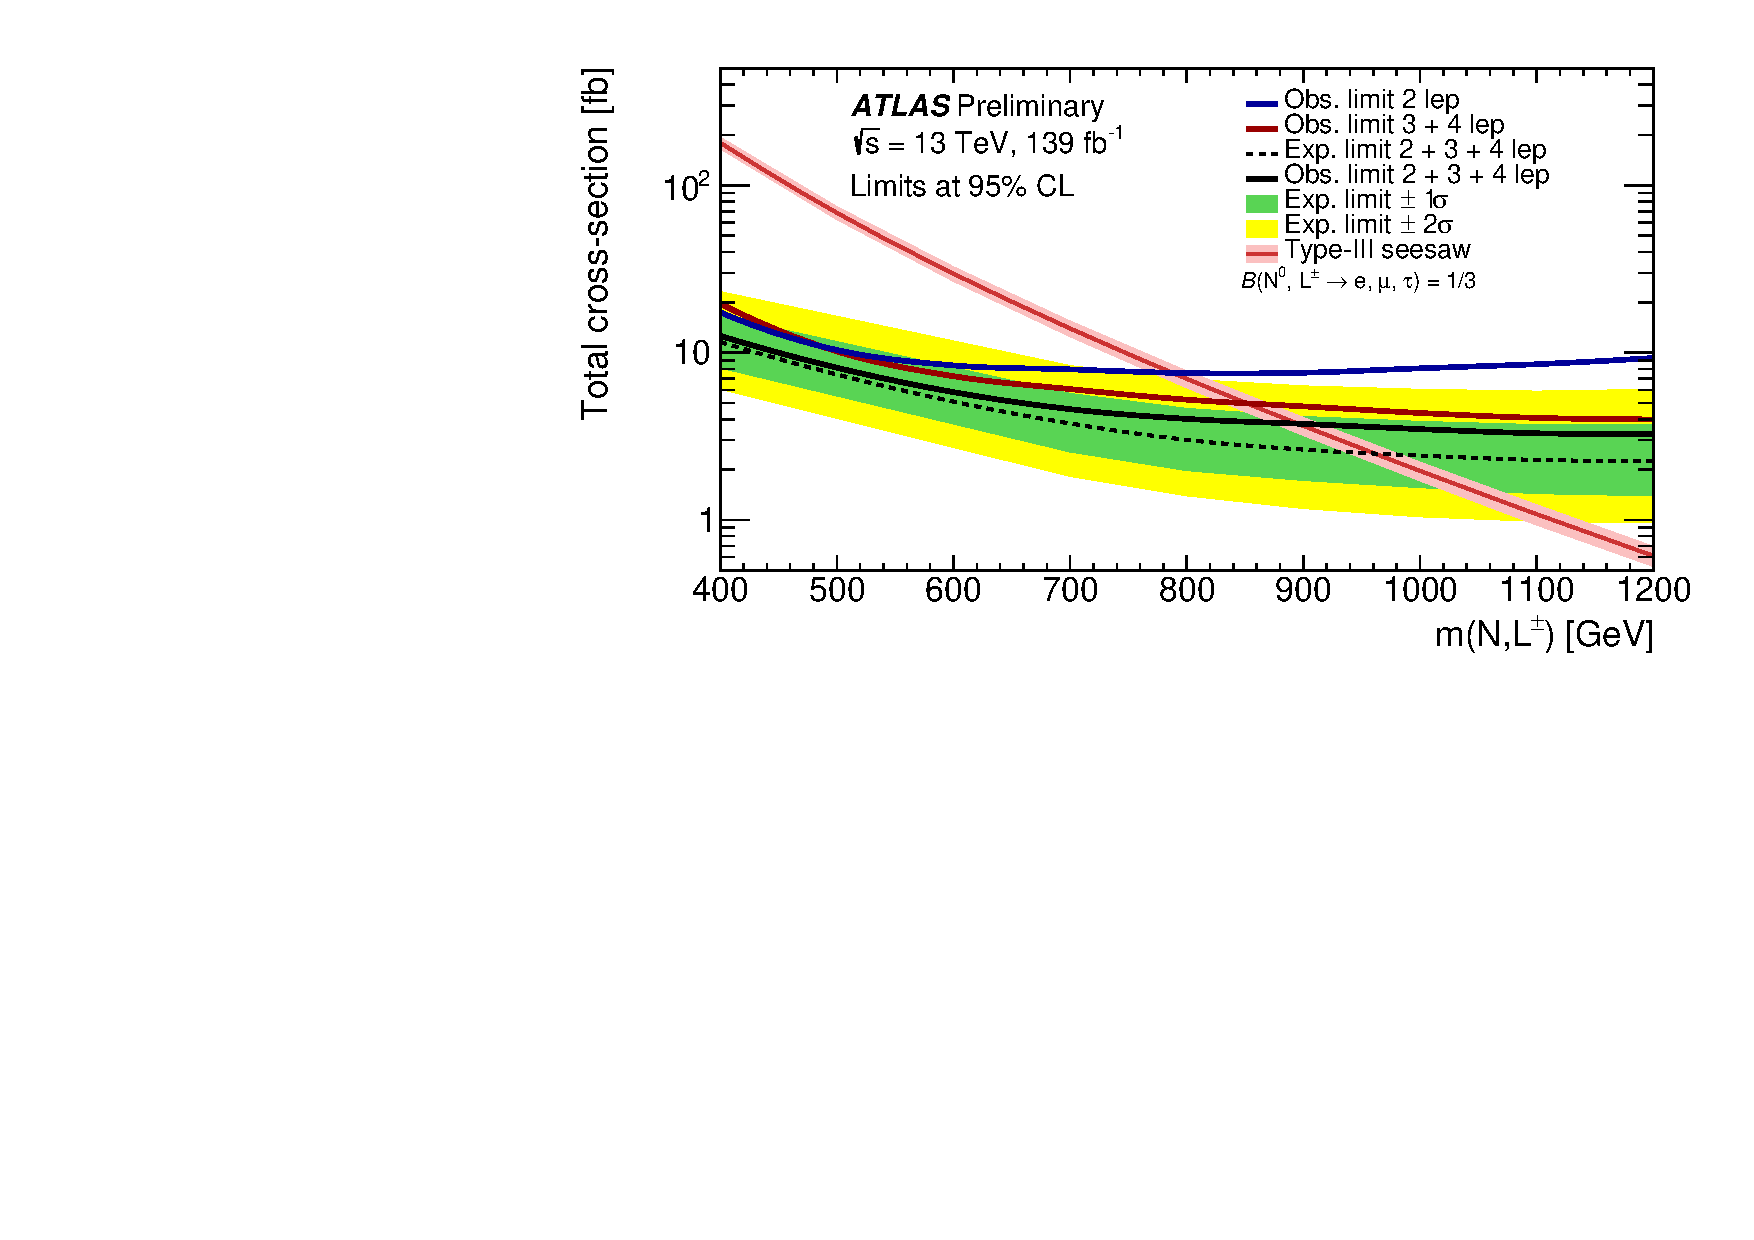
\includegraphics[width=0.7\textwidth]{ATLAS-CONF-2021-023.pdf}
\caption{\label{fig:ATLAS-CONF-2021-023}Expected and observed CLs upper limits on the cross section for the type-III seesaw process. Figure taken from Ref.~\cite{ATLAS-CONF-2021-023}.}
\end{center}
\end{figure}

The LHCb collaboration conducted a search for HNLs in $\textrm{W}\to\mu\mu$+jets events~\cite{LHCb-PAPER-2020-022}. The analysis targets simultaneously Dirac or Majorana HNLs in the mass range of 5--50~GeV. The branching fraction, $\mathcal{B}(N\to\mu\,\textrm{jets})|V_{\mu N}|^2$, of HNL production is determined by measuring the ratio with respect to $\textrm{W}\to\mu\nu$ production. Upper limits on the coupling are presented in Fig.~\ref{fig:LHCb-PAPER-2020-022} as a function of the HNL mass, which are obtained by assuming a branching fraction of 0.51 and no couplings to electrons or taus.

\begin{figure}[htbp]
\begin{center}
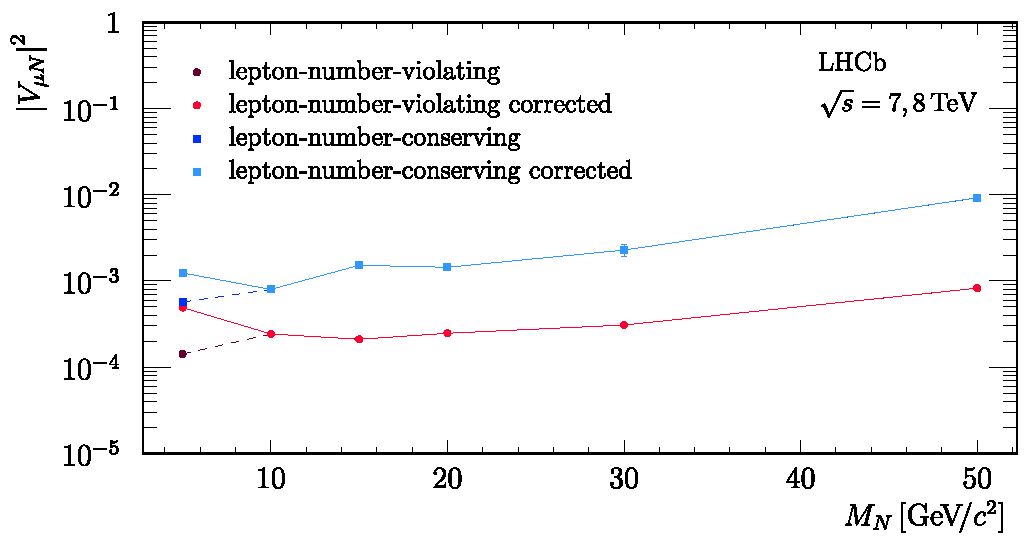
\includegraphics[width=0.6\textwidth]{LHCb-PAPER-2020-022.pdf}
\caption{\label{fig:LHCb-PAPER-2020-022}Observed upper limit on the mixing parameter $|V_{\mu N}|^2$ between a heavy neutrino and a muon neutrino. Figure taken from Ref.~\cite{LHCb-PAPER-2020-022}.}
\end{center}
\end{figure}

A generic search for long-lived particles (LLPs) with decays to $\textrm{e}^{\pm}\mu^{\mp}\nu$ final states has also been performed by the LHCb collaboration~\cite{LHCb-PAPER-2020-027}. The resulting upper limits for direct LLP pair production (DPP), SM Higgs with decays to LLP pairs, and charge current (CC) production are shown in Fig.~\ref{fig:LHCb-PAPER-2020-027}.

\begin{figure}[htbp]
\begin{center}
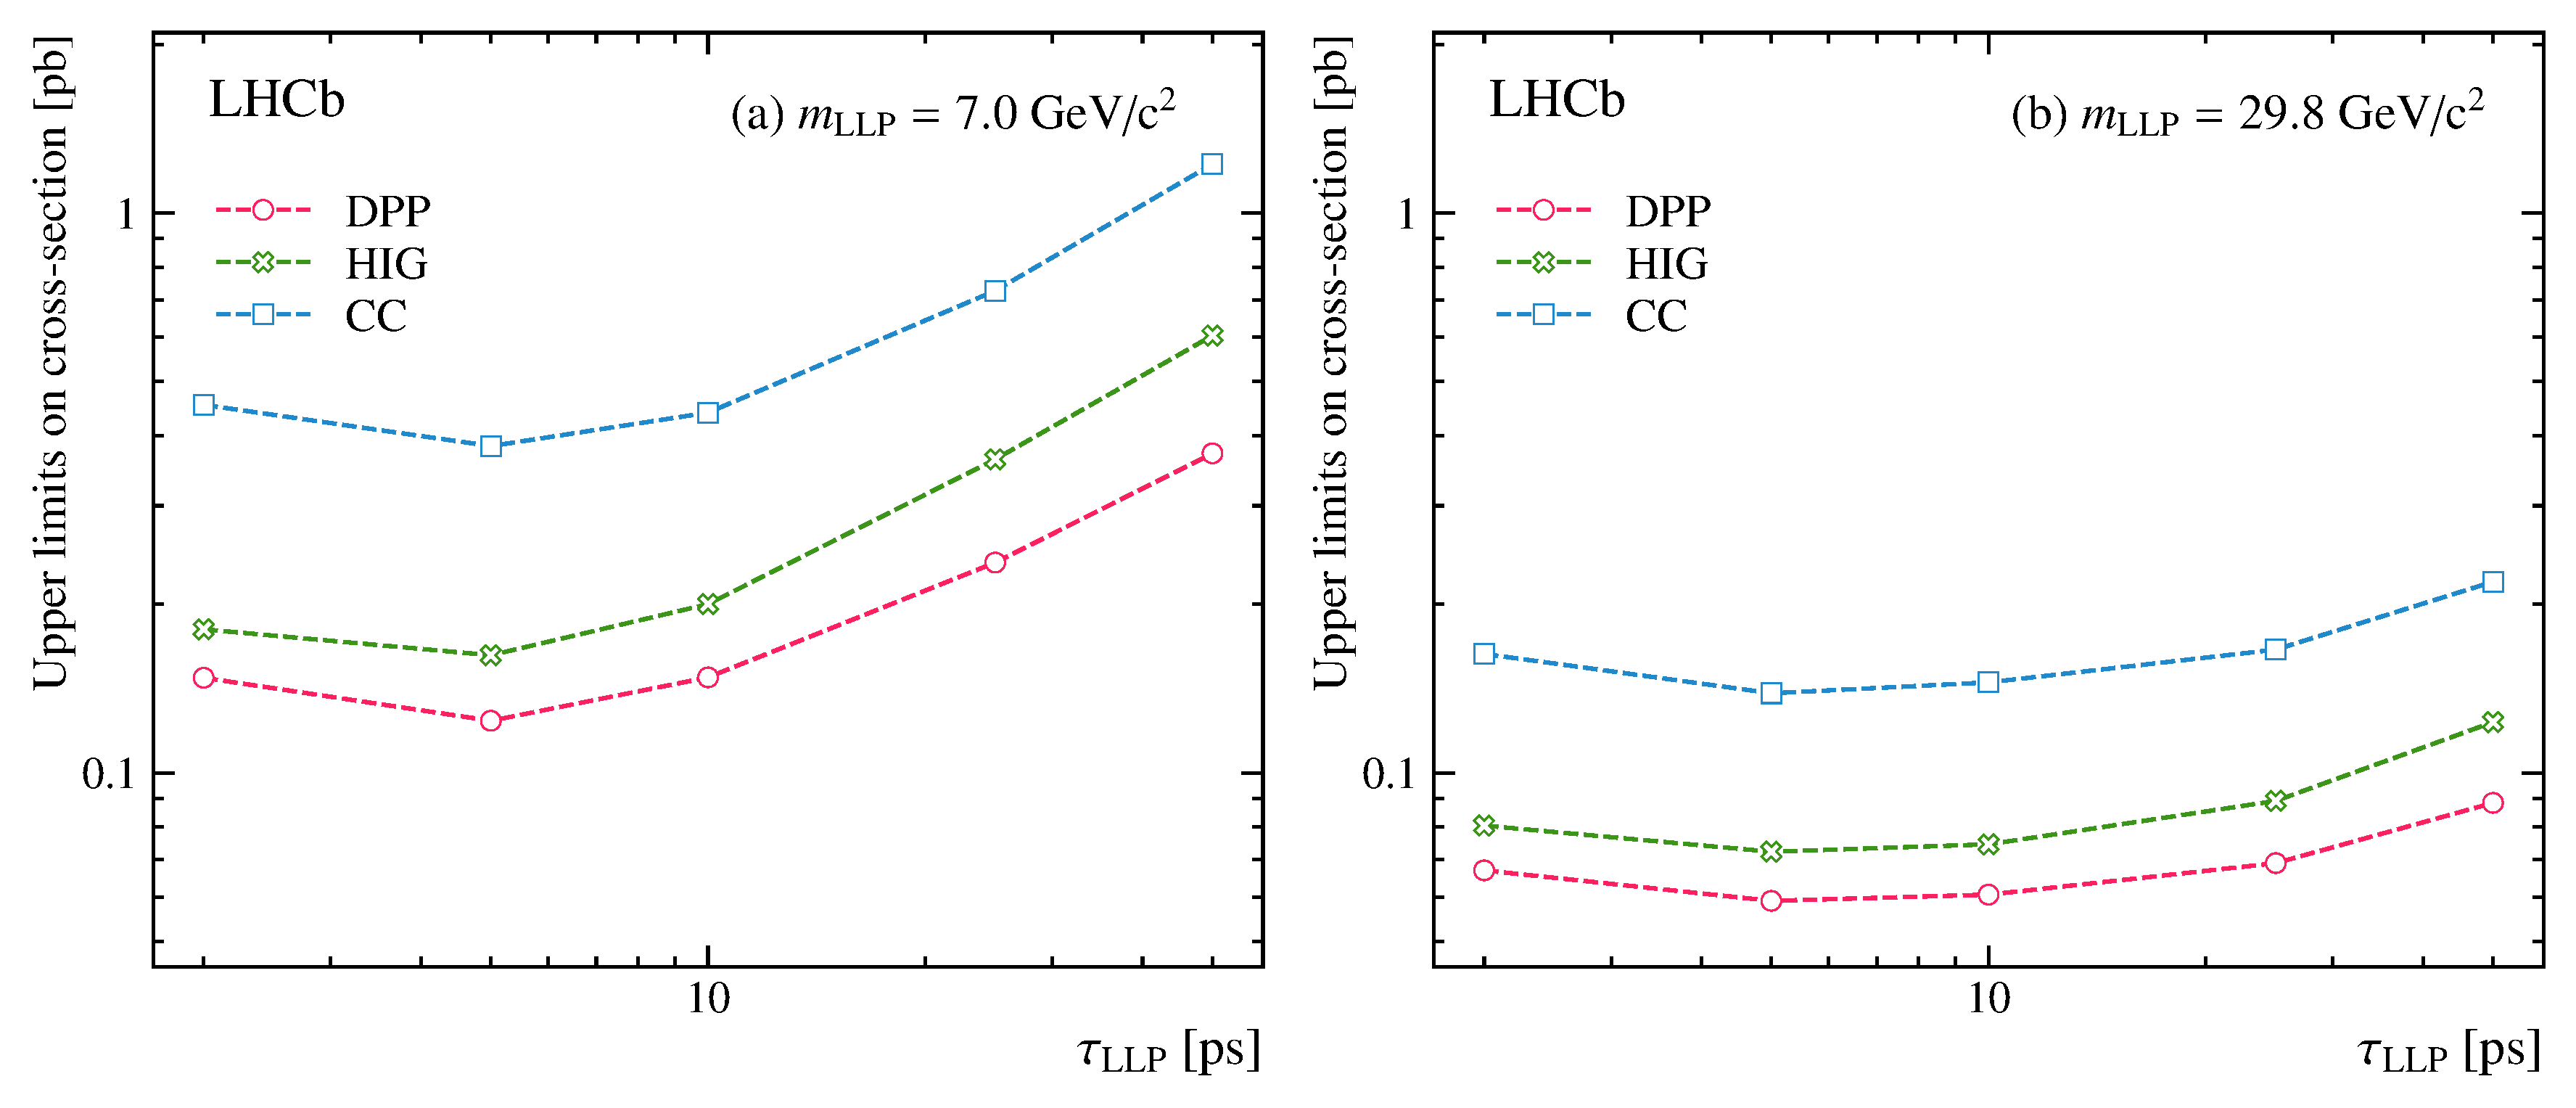
\includegraphics[width=0.7\textwidth]{LHCb-PAPER-2020-027.pdf}
\caption{\label{fig:LHCb-PAPER-2020-027}Observed upper limits on the production cross-sections times branching fraction for (left)~$m_{LLP}=7$~GeV and (right)~$m_{LLP}=29.8$~GeV as function of the HNL proper lifetime. Figure taken from Ref.~\cite{LHCb-PAPER-2020-027}.}
\end{center}
\end{figure}

\section{Summary}
A comprehensive search programme for heavy neutral leptons is being conducted at the LHC. The probed models include prompt HNLs with and without flavour-violating decays, righted-handed W~bosons, type-III seesaw, and long-lived HNLs besides others.


\begin{thebibliography}{99}

\bibitem{pheno}{K. Bondarenko, et al., \emph{Phenomenology of GeV-scale heavy neutral leptons}, \emph{JHEP}~\textbf{11} (2018) 032, {\tt arXiv:1805.08567\,[hep-ph]}.}

\bibitem{llp1}{ATLAS Collaboration, \emph{Search for heavy neutral leptons in decays of $W$ bosons produced in 13~TeV $pp$ collisions using prompt and displaced signatures with the ATLAS detector}, \emph{JHEP}~\textbf{10} (2019) 265, {\tt  arXiv:1905.09787\,[hep-ex]}.}

\bibitem{llp2}{CMS Collaboration, \emph{Search for heavy Majorana neutrinos in same-sign dilepton channels in proton-proton collisions at $\sqrt{s}=$~13\,TeV}, \emph{JHEP}~\textbf{01} (2019) 122, {\tt arXiv:1806.10905\,[hep-ex]}.}

\bibitem{llp3}{CMS Collaboration, \emph{Search for heavy neutral leptons in events with three charged leptons in proton-proton collisions at $\sqrt{s} =$~13\,TeV}, \emph{Phys. Rev. Lett.}~\textbf{120} (2018) 22, 221801, {\tt arXiv:1802.02965\,[hep-ex]}.}

\bibitem{atlas}{ATLAS Collaboration, \emph{The ATLAS Experiment at the CERN Large Hadron Collider}, \emph{JINST}~\textbf{3} (2008) S08003.}
\bibitem{cms}{CMS Collaboration, \emph{The CMS experiment at the CERN LHC}, \emph{JINST}~\textbf{3} (2008) S08004.}
\bibitem{lhcb}{LHCB Collaboration, \emph{The LHCb Detector at the LHC}, \emph{JINST}~\textbf{3} (2008) S08005.}

\bibitem{wr1}{CMS Collaboration, \emph{Search for a heavy right-handed W boson and a heavy neutrino in events with two same-flavor leptons and two jets at $\sqrt{s}=$~13\,TeV}, \emph{JHEP}~\textbf{05} (2018) 148, {\tt arXiv:1803.11116\,[hep-ex]}.} 

\bibitem{wr2}{CMS Collaboration, \emph{Search for heavy neutrinos and third-generation leptoquarks in hadronic states of two $\tau$ leptons and two jets in proton-proton collisions at $\sqrt{s} =$~13\,TeV}, \emph{JHEP}~\textbf{03} (2019) 170, {\tt arXiv:1811.00806\,[hep-ex]}.}

\bibitem{wr3}{ATLAS Collaboration, \emph{Search for heavy Majorana or Dirac neutrinos and right-handed $W$ gauge bosons in final states with two charged leptons and two jets at $ \sqrt{s}=$~13\,TeV with the ATLAS detector}, \emph{JHEP}~\textbf{01} (2019) 016, {\tt arXiv:1809.11105\,[hep-ex]}.}

\bibitem{wr4}{ATLAS Collaboration, \emph{Search for a right-handed gauge boson decaying into a high-momentum heavy neutrino and a charged lepton in $pp$ collisions with the ATLAS detector at $\sqrt{s}=$~13\,TeV}, \emph{Phys. Lett. B}~\textbf{798} (2019) 134942, {\tt arXiv:1904.12679\,[hep-ex]}.}

\bibitem{ATLAS-CONF-2021-023}{ATLAS Collaboration, \emph{Search for type-III seesaw heavy leptons in leptonic final states in $pp$ collisions at $\sqrt {s}=$~13\,TeV with the ATLAS detector}, ATLAS-CONF-2021-023, 2021.}

\bibitem{LHCb-PAPER-2020-022}{LHCb Collaboration, \emph{Search for heavy neutral leptons in $W^+\to\mu^{+}\mu^{\pm}\text{jet}$ decays}, \emph{Eur. Phys. J. C}~\textbf{81} (2021) 3, 248, {\tt arXiv:2011.05263\,[hep-ex]}.}

\bibitem{LHCb-PAPER-2020-027}{LHCb Collaboration, \emph{Search for long-lived particles decaying to $e^\pm \mu^\mp \nu$}, \emph{Eur. Phys. J. C}~\textbf{81} (2021) 3, 261, {\tt arXiv:2012.02696\,[hep-ex]}.}

\end{thebibliography}

\end{document}
